\chapter{Genomic sequence tools}
\label{gst}

Current available genomic sequence tools, for analysis and manipulation, are:
\begin{enumerate}

\item \texttt{gto\char`_genomic\char`_gen\char`_random\char`_dna}: it generates a synthetic DNA.

\item \texttt{gto\char`_genomic\char`_rand\char`_seq\char`_extra\char`_chars}: it substitues in the DNA sequence the outside ACGT chars by random ACGT symbols.

\item \texttt{gto\char`_genomic\char`_dna\char`_mutate}: it creates a synthetic mutation of a sequence file given specific rates of mutations, deletions and additions.

\item \texttt{gto\char`_genomic\char`_extract}: it extracts sequences from a sequence file, which the range is defined by the user in the parameters.

\item \texttt{gto\char`_genomic\char`_period}: it calculates the best order depth of a sequence, using FCMs.
\end{enumerate}

\section{Program gto\char`_genomic\char`_gen\char`_random\char`_dna}
The \texttt{gto\char`_genomic\char`_gen\char`_random\char`_dna} generates a synthetic DNA.\\
For help type:
\begin{lstlisting}
./gto_genomic_gen_random_dna -h
\end{lstlisting}
In the following subsections, we explain the input and output paramters.

\subsection*{Input parameters}

The \texttt{gto\char`_genomic\char`_gen\char`_random\char`_dna} program needs one stream for the computation, namely the output standard.\\
The attribution is given according to:
\begin{lstlisting}
Usage: ./gto_genomic_gen_random_dna [options] [[--] args]
   or: ./gto_genomic_gen_random_dna [options]

It generates a synthetic DNA.

    -h, --help                show this help message and exit

Basic options
    > output.seq              Output synthetic DNA sequence (stdout)

Optional
    -s, --seed=<int>          Starting point to the random generator (Default 0)
    -n, --nSymbols=<int>      Number of symbols generated (Default 100)
    -f, --frequency=<str>     The frequency of each base. It should be represented 
    						  in the following format: <fa,fc,fg,ft>.

Example: ./gto_genomic_gen_random_dna > output.seq
\end{lstlisting}

\subsection*{Output}
The output of the \texttt{gto\char`_genomic\char`_gen\char`_random\char`_dna} program is a sequence group file whith the synthetic DNA.\\
Using the input above with the seed value as 1 and the number of symbols as 400, an output example for this is the following:
\begin{lstlisting}
TCTTTACTCGCGCGTTGGAGAAATACAATAGTGCGGCTCTGTCTCCTTATGAAGTCAACAATTTCGCTGGGACTTGCGGC
TCTTTACTCGCGCGTTGGAGAAATACAATAGTGCGGCTCTGTCTCCTTATGAAGTCAACAATTTCGCTGGGACTTGCGGC
GACTTCATCGTGGTCTCTGTCATTATGCGCTCCAACGCATAACTTTGCGCCAGAAGATAGATAGAATGGTGTAAGAAACT
GTAATATATATAATGAACTTCGGCGAGTCTGTGGAGTTTTTGTTGCATTAGAGAGCCAAGAGGTCGGACGTCCTCACGTA
GCCCGAGACGGGCAGGGCGATGGCGACTGAACGGGCTCCATATCACTTTGAGCTTTTATGCTTTCGACTCCTCCAGGAGC
TGAACAACCTTGTTCCCGGCAAAGCCCACTGCGTCATGGAGCTCACGGTCTACATTCATGACTGACTAACCGTAAACTGC
\end{lstlisting}

\section{Program gto\char`_genomic\char`_rand\char`_seq\char`_extra\char`_chars}
The \texttt{gto\char`_genomic\char`_rand\char`_seq\char`_extra\char`_chars} substitues in the DNA sequence the outside ACGT chars by random ACGT symbols. It works in sequence file formats.\\
For help type:
\begin{lstlisting}
./gto_genomic_rand_seq_extra_chars -h
\end{lstlisting}
In the following subsections, we explain the input and output paramters.

\subsection*{Input parameters}

The \texttt{gto\char`_genomic\char`_rand\char`_seq\char`_extra\char`_chars} program needs two streams for the computation, namely the input and output standard. The input stream is a sequence file.\\
The attribution is given according to:
\begin{lstlisting}
Usage: ./gto_genomic_rand_seq_extra_chars [options] [[--] args]
   or: ./gto_genomic_rand_seq_extra_chars [options]

It substitues in the DNA sequence the outside ACGT chars by random ACGT symbols.
It works in sequence file formats


    -h, --help        show this help message and exit

Basic options
    < input.seq       Input sequence file (stdin)
    > output.seq      Output sequence file (stdout)

Example: ./gto_genomic_rand_seq_extra_chars < input.seq > output.seq
\end{lstlisting}
An example on such an input file is:
\begin{lstlisting}
ANAAGACGNNNTCCTGCTGCTGCTGCTCTCCGGGGCCACGGCCCTGGAGGGTCCACCGCTGCCCTGCTGCCATTGTCCCC
NNCCCCACCTAAGGAAAAGCAGCCTCCTGACTTTCCTCGCTTGGGCCGAGACAGCGAGCATATGCAGGAAGCGGCAGGAA
GTGGTTTGAGTGGACCTCCGGGCCCCNNNNNGGAGAGGAAGCTCGGGAGNGTNNNGGCCAGGCGGCAGNNNNCCAGTGCC
GCGAATCCGCGCGCCGGGACAGAATCTCCTGCAAAGCCCTGCAGGAACTTCTTCTGGAAGACCTTCTCCACCCCCCCAGC
TANNNNCTCACCCATGAATGCTCACGCAAGTTTAATTACAGACCTGAAACAAGATGCCATTGTCCCCCGGCCTCCTGCTG
CTGCTGCTCTCCGGGGCCACGGCCACCGCTGCCCTGCCCCTGGAGGGTGGCCCCACCGGCCGAGACAGCGAGCATATGCA
GGAAGCGGCAGGAATAAGNNNAAGCAGCCTCCTGACTTTCCTCGCTTGNNNNTTTGAGTGGACCTCCCAGGCCAGTGCCG
GGCCCCTCATAGGAGAGGAAGCTCGGGAGGTGGCCAGGCGGCAGGAAGGCGCACCCCCCCAGCAATCCGCGCGCCGGGAC
AGAATGCCCTGCAGGAACTTCTTCTGGAAGACCTTCTCCTCCTGCAAATAAAACCTCACCCATGAATGCTCACGCAAGTT
NNATTACNNNCCTGNN
\end{lstlisting}

\subsection*{Output}
The output of the \texttt{gto\char`_genomic\char`_rand\char`_seq\char`_extra\char`_chars} program is a sequence file.\\
Using the input above, an output example for this is the following:
\begin{lstlisting}
ATAAGACGGCTTCCTGCTGCTGCTGCTCTCCGGGGCCACGGCCCTGGAGGGTCCACCGCTGCCCTGCTGCCATTGTCCCC
CTCCCCACCTAAGGAAAAGCAGCCTCCTGACTTTCCTCGCTTGGGCCGAGACAGCGAGCATATGCAGGAAGCGGCAGGAA
GTGGTTTGAGTGGACCTCCGGGCCCCGACCGGGAGAGGAAGCTCGGGAGTGTGTTGGCCAGGCGGCAGGAGACCAGTGCC
GCGAATCCGCGCGCCGGGACAGAATCTCCTGCAAAGCCCTGCAGGAACTTCTTCTGGAAGACCTTCTCCACCCCCCCAGC
TAATATCTCACCCATGAATGCTCACGCAAGTTTAATTACAGACCTGAAACAAGATGCCATTGTCCCCCGGCCTCCTGCTG
CTGCTGCTCTCCGGGGCCACGGCCACCGCTGCCCTGCCCCTGGAGGGTGGCCCCACCGGCCGAGACAGCGAGCATATGCA
GGAAGCGGCAGGAATAAGCGGAAGCAGCCTCCTGACTTTCCTCGCTTGGTTTTTTGAGTGGACCTCCCAGGCCAGTGCCG
GGCCCCTCATAGGAGAGGAAGCTCGGGAGGTGGCCAGGCGGCAGGAAGGCGCACCCCCCCAGCAATCCGCGCGCCGGGAC
AGAATGCCCTGCAGGAACTTCTTCTGGAAGACCTTCTCCTCCTGCAAATAAAACCTCACCCATGAATGCTCACGCAAGTT
CGATTACGGCCCTGTC
\end{lstlisting}
\section{Program gto\char`_genomic\char`_dna\char`_mutate}
The \texttt{gto\char`_genomic\char`_dna\char`_mutate} creates a synthetic mutation of a sequence file given specific rates of mutations, deletions and additions. All these paramenters are defined by the user, and their are optional.\\
For help type:
\begin{lstlisting}
./gto_genomic_dna_mutate -h
\end{lstlisting}
In the following subsections, we explain the input and output paramters.

\subsection*{Input parameters}

The \texttt{gto\char`_genomic\char`_dna\char`_mutate} program needs two streams for the computation, namely the input and output standard. However, optional settings can be supplied too, such as the starting point to the random generator, and the edition, deletion and insertion rates. Also, the user can choose to use the ACGTN alphabet in the synthetic mutation. The input stream is a sequence File.\\
The attribution is given according to:
\begin{lstlisting}
Usage: ./gto_genomic_dna_mutate [options] [[--] args]
   or: ./gto_genomic_dna_mutate [options]

Creates a synthetic mutation of a sequence file given specific rates of mutations, 
deletions and additions

    -h, --help                    show this help message and exit

Basic options
    < input.seq                   Input sequence file (stdin)
    > output.seq                  Output sequence file (stdout)

Optional
    -s, --seed=<int>              Starting point to the random generator
    -m, --mutation-rate=<dbl>     Defines the mutation rate (default 0.0)
    -d, --deletion-rate=<dbl>     Defines the deletion rate (default 0.0)
    -i, --insertion-rate=<dbl>    Defines the insertion rate (default 0.0)
    -a, --ACGTN-alphabet          When active, the application uses the ACGTN alphabet

Example: ./gto_genomic_dna_mutate -s <seed> -m <mutation rate> -d <deletion rate> -i 
<insertion rate> -a < input.seq > output.seq
\end{lstlisting}
An example on such an input file is:
\begin{lstlisting}
TCTTTACTCGCGCGTTGGAGAAATACAATAGTGCGGCTCTGTCTCCTTATGAAGTCAACAATTTCGCTGGGACTTGCGGC
TCTTTACTCGCGCGTTGGAGAAATACAATAGTGCGGCTCTGTCTCCTTATGAAGTCAACAATTTCGCTGGGACTTGCGGC
GACTTCATCGTGGTCTCTGTCATTATGCGCTCCAACGCATAACTTTGCGCCAGAAGATAGATAGAATGGTGTAAGAAACT
GTAATATATATAATGAACTTCGGCGAGTCTGTGGAGTTTTTGTTGCATTAGAGAGCCAAGAGGTCGGACGTCCTCACGTA
GCCCGAGACGGGCAGGGCGATGGCGACTGAACGGGCTCCATATCACTTTGAGCTTTTATGCTTTCGACTCCTCCAGGAGC
TGAACAACCTTGTTCCCGGCAAAGCCCACTGCGTCATGGAGCTCACGGTCTACATTCATGACTGACTAACCGTAAACTGC
\end{lstlisting}

\subsection*{Output}
The output of the \texttt{gto\char`_genomic\char`_dna\char`_mutate} program is a sequence file whith the synthetic mutation of input file.\\
Using the seed value as 1 and the mutation rate as 0.5, an example for this input, is: 
\begin{lstlisting}
TCACGACTGTCGCGTTGGCACACCAGATAGGTGCTTCTACGTTTTGTATCTAATTTACAATTCTCGCTGGGAGTTCATTC
GCTATTGATGGGACTAGAAACCCATCCGTAGCTTGCCGCCGTTTAAGAATAAACACTCCACTTGCACCGAGACGTAGCGC
AACCAAGGCTATGTTCTTTGACCTTATGCGGTCCAACGCAGGAGTAGACCCCCGTAGTTAGGTACTATCGCAGAATAGGC
TTAAGCAGCCGTGCTGAACGCTGGAGGGTCTGTTTAATTACTGAGTGAATGGAGAGCTAAGAGTTCGGAGCACCGCACGA
GGCTCAAGAGCGGAAGGGCGTCAGCCTGGCGACCACCTGCCTACCGCTCGAGTCTGTCTTCACTACAGTCCGTGGAGGAC
CCCCAACGACCTAGTATCCTACAAAGCCGCATACGACTTACAGAACAGGCTGTATCGTCAGGAGTGTGTACACGAAGAGT
A
\end{lstlisting}

\section{Program gto\char`_genomic\char`_extract}
The \texttt{gto\char`_genomic\char`_extract} extracts sequences from a sequence file, which the range is defined by the user in the parameters.\\
For help type:
\begin{lstlisting}
./gto_genomic_extract -h
\end{lstlisting}
In the following subsections, we explain the input and output paramters.

\subsection*{Input parameters}

The \texttt{gto\char`_genomic\char`_extract} program needs two paramenters, which defines the begin and the end of the extraction, and two streams for the computation, namely the input and output standard. The input stream is a sequence file.\\
The attribution is given according to:
\begin{lstlisting}
Usage: ./gto_genomic_extract [options] [[--] args]
   or: ./gto_genomic_extract [options]

It extracts sequences from a sequence file.

    -h, --help        show this help message and exit

Basic options
    -i, --init=<int>  The first position to start the extraction (default 0)
    -e, --end=<int>   The last extract position (default 100)
    < input.seq       Input sequence file (stdin)
    > output.seq      Output sequence file (stdout)

Example: ./gto_genomic_extract -i <init> -e <end> < input.seq > output.seq
\end{lstlisting}
An example on such an input file is:
\begin{lstlisting}
TCTTTACTCGCGCGTTGGAGAAATACAATAGTGCGGCTCTGTCTCCTTATGAAGTCAACAATTTCGCTGGGACTTGCGGC
TCTTTACTCGCGCGTTGGAGAAATACAATAGTGCGGCTCTGTCTCCTTATGAAGTCAACAATTTCGCTGGGACTTGCGGC
GACTTCATCGTGGTCTCTGTCATTATGCGCTCCAACGCATAACTTTGCGCCAGAAGATAGATAGAATGGTGTAAGAAACT
GTAATATATATAATGAACTTCGGCGAGTCTGTGGAGTTTTTGTTGCATTAGAGAGCCAAGAGGTCGGACGTCCTCACGTA
GCCCGAGACGGGCAGGGCGATGGCGACTGAACGGGCTCCATATCACTTTGAGCTTTTATGCTTTCGACTCCTCCAGGAGC
TGAACAACCTTGTTCCCGGCAAAGCCCACTGCGTCATGGAGCTCACGGTCTACATTCATGACTGACTAACCGTAAACTGC
\end{lstlisting}

\subsection*{Output}
The output of the \texttt{gto\char`_genomic\char`_extract} program is a group sequence.\\
An example, using the value 0 as extraction starting point and the 50 as the end, for the provided input, is:
\begin{lstlisting}
TCTTTACTCGCGCGTTGGAGAAATACAATAGTGCGGCTCTGTCTCCTTAT
\end{lstlisting}
\section{Program gto\char`_genomic\char`_period}
The \texttt{gto\char`_genomic\char`_period} calculates the best order depth of a sequence, using FCMs. It only works "ACGT", while the rest will be discarded.\\
This application has a dependency to represent the results. It requires the Gnuplot to show the execution result.\\
For help type:
\begin{lstlisting}
./gto_genomic_period -h
\end{lstlisting}
In the following subsections, we explain the input and output paramters.

\subsection*{Input parameters}

The \texttt{gto\char`_genomic\char`_period} program needs program needs two streams for the computation, namely the input and output standard. The input stream is a sequence file.\\
The attribution is given according to:
\begin{lstlisting}
Usage: ./gto_genomic_period [options] [[--] args]
   or: ./gto_genomic_period [options]

It calculates the best order depth of a sequence, using FCMs.It only works "ACGT", 
while the rest will be discarded.

    -h, --help        show this help message and exit

Basic options
    < input.seq       Input sequence file format (stdin)
    > output          Output is given by log_2(4)*K(x)/|x|) (stdout)

Example: ./gto_genomic_period < input.seq > output
\end{lstlisting}
An example on such an input file is:
\begin{lstlisting}
TCTTTACTCGCGCGTTGGAGAAATACAATAGTGCGGCTCTGTCTCCTTATGAAGTCAACAATTTCGCTGGGACTTGCGGC
TCTTTACTCGCGCGTTGGAGAAATACAATAGTGCGGCTCTGTCTCCTTATGAAGTCAACAATTTCGCTGGGACTTGCGGC
GACTTCATCGTGGTCTCTGTCATTATGCGCTCCAACGCATAACTTTGCGCCAGAAGATAGATAGAATGGTGTAAGAAACT
GTAATATATATAATGAACTTCGGCGAGTCTGTGGAGTTTTTGTTGCATTAGAGAGCCAAGAGGTCGGACGTCCTCACGTA
GCCCGAGACGGGCAGGGCGATGGCGACTGAACGGGCTCCATATCACTTTGAGCTTTTATGCTTTCGACTCCTCCAGGAGC
TGAACAACCTTGTTCCCGGCAAAGCCCACTGCGTCATGGAGCTCACGGTCTACATTCATGACTGACTAACCGTAAACTGC
\end{lstlisting}

\subsection*{Output}
The output of the \texttt{gto\char`_genomic\char`_period} program is a execution report, followed by the plot with this information.\\
An example of the report, for the input, is:
\begin{lstlisting}
Running order: 1 ... Done!
Running order: 2 ... Done!
Running order: 3 ... Done!
Running order: 4 ... Done!
Running order: 5 ... Done!
Running order: 6 ... Done!
Running order: 7 ... Done!
Running order: 8 ... Done!
Running order: 9 ... Done!
Running order: 10 ... Done!
Running order: 11 ... Done!
Running order: 12 ... Done!
Running order: 13 ... Done!
Running order: 14 ... Done!
Running order: 15 ... Done!
Running order: 16 ... Done!
Running order: 17 ... Done!
Running order: 18 ... Done!
Running order: 19 ... Done!
Running order: 20 ... Done!
 1	2.246
 2	2.225
 3	2.237
 4	2.079
 5	1.821
 6	1.733
 7	1.717
 8	1.708
 9	1.717
10	1.712
11	1.717
12	1.721
13	1.725
14	1.729
15	1.733
16	1.738
17	1.742
18	1.746
19	1.75
20	1.754
\end{lstlisting}

In the Figure~\ref{fig:gtoGenomicPeriod} is represented the plot for the execution above.

 \begin{figure}[!h]
  \centering
  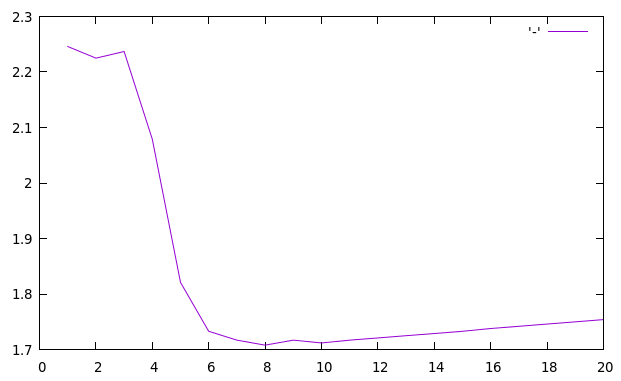
\includegraphics[scale=0.7]{./images/gto_genomic_period.png}
  \caption{\texttt{gto\char`_genomic\char`_period} execution plot.}
  \label{fig:gtoGenomicPeriod}
 \end{figure}
